\documentclass{article}



\usepackage{arxiv}

\usepackage[utf8]{inputenc} % allow utf-8 input
\usepackage[T1]{fontenc}    % use 8-bit T1 fonts
\usepackage{hyperref}       % hyperlinks
\usepackage{url}            % simple URL typesetting
\usepackage{booktabs}       % professional-quality tables
\usepackage{amsfonts}       % blackboard math symbols
\usepackage{nicefrac}       % compact symbols for 1/2, etc.
\usepackage{microtype}      % microtypography
\usepackage{lipsum}		% Can be removed after putting your text content
\usepackage{graphicx}
\usepackage{natbib}
\usepackage{doi}
\usepackage[noend]{algpseudocode}
\usepackage{amsmath}
\usepackage{algorithm}
\usepackage{algorithmicx}


\renewcommand{\algorithmicrequire}{\textbf{Input:}}  % Use Input in the format of Algorithm  
\renewcommand{\algorithmicensure}{\textbf{Output:}} % Use Output in the format of Algorithm  


\title{Boosting Monocular 3D Object Detection through Depth Probabilistic Optimization}

%\date{September 9, 1985}	% Here you can change the date presented in the paper title
%\date{} 					% Or removing it

\author{ \href{https://orcid.org/0000-0002-2277-8871}{
\includegraphics[scale=0.06]{orcid.pdf}\hspace{1mm}Tingyu Zhang}\thanks{Use footnote for providing further
		information about author (webpage, alternative
		address)---\emph{not} for acknowledging funding agencies.} \\
	College of Computer Science and Technology\\
	Jilin University\\
	Chang Chun, Jilin \\
	\texttt{zhangty21@mails.jlu.edu.cn} \\
	%% examples of more authors
	\And
	\href{https://orcid.org/0000-0002-7701-8511}{
\includegraphics[scale=0.06]{orcid.pdf}\hspace{1mm}Jian Wang} \\
	College of Computer Science and Technology\\
	Jilin University\\
	Chang Chun, Jilin \\
	\texttt{wangjian591@jlu.edu.cn} \\
	%% \AND
	%% Coauthor \\
	%% Affiliation \\
	%% Address \\
	%% \texttt{email} \\
	%% \And
	%% Coauthor \\
	%% Affiliation \\
	%% Address \\
	%% \texttt{email} \\
	%% \And
	%% Coauthor \\
	%% Affiliation \\
	%% Address \\
	%% \texttt{email} \\
}

% Uncomment to remove the date
%\date{}

% Uncomment to override  the `A preprint' in the header
%\renewcommand{\headeright}{Technical Report}
%\renewcommand{\undertitle}{Technical Report}
\renewcommand{\shorttitle}{\textit{arXiv} Template}

%%% Add PDF metadata to help others organize their library
%%% Once the PDF is generated, you can check the metadata with
%%% $ pdfinfo template.pdf
\hypersetup{
pdftitle={A template for the arxiv style},
pdfsubject={q-bio.NC, q-bio.QM},
pdfauthor={David S.~Hippocampus, Elias D.~Striatum},
pdfkeywords={First keyword, Second keyword, More},
}


\begin{document}
\maketitle

\begin{abstract}
	\lipsum[1]
\end{abstract}


% keywords can be removed
\keywords{First keyword \and Second keyword \and More}
\begin{figure}[!t]
	\centering
	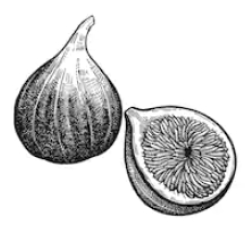
\includegraphics[width=1.0\linewidth]{Figures/fig1}
	\caption{None}
	\label{fig:overview}
\end{figure}

\begin{figure}[!t]
	\centering
	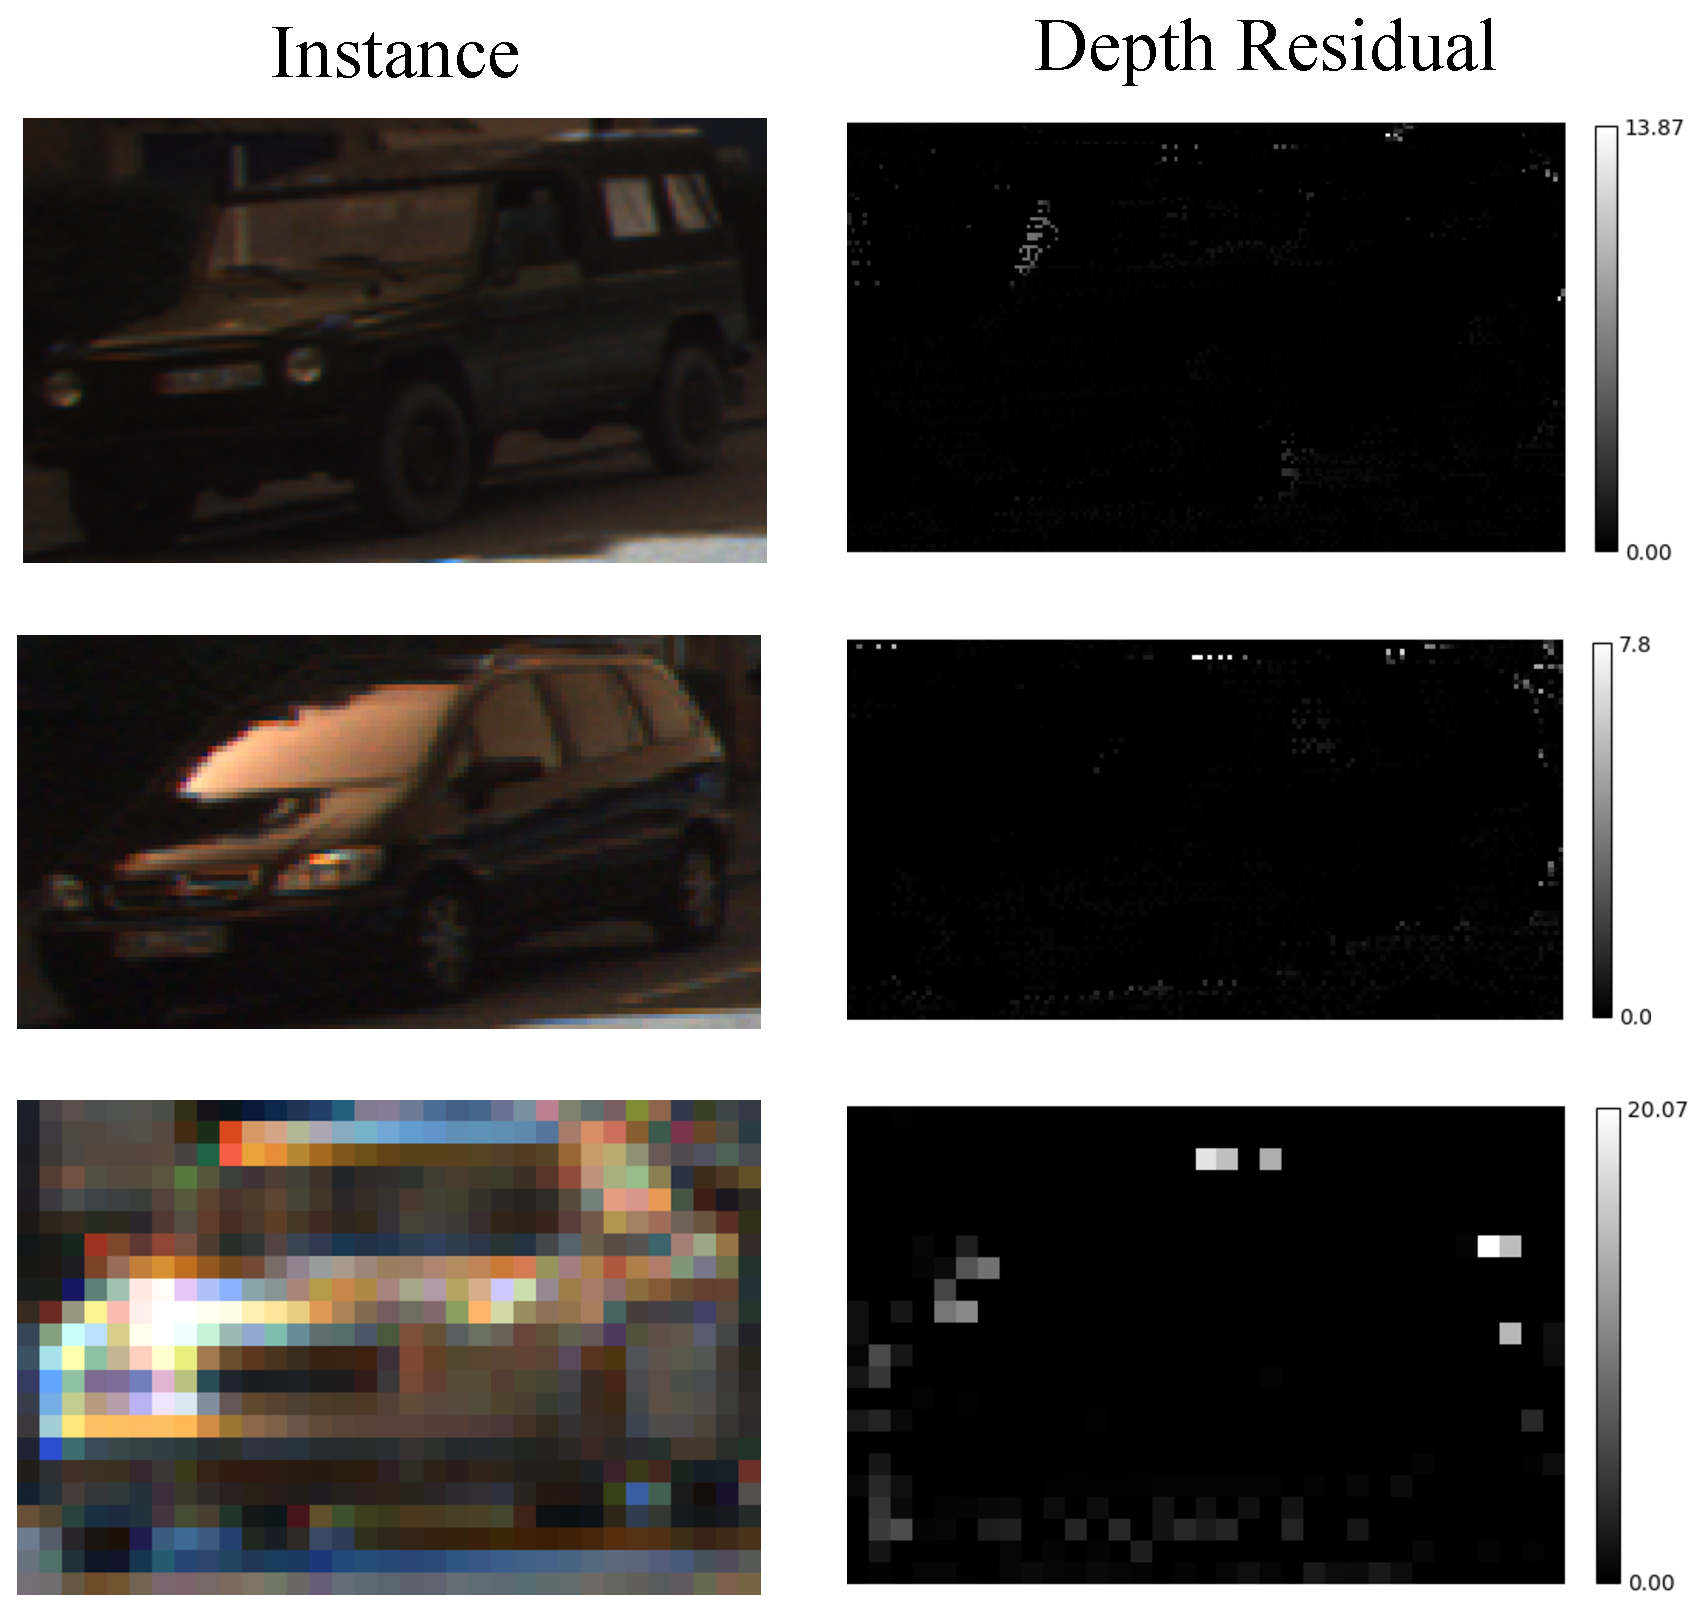
\includegraphics[width=1.0\linewidth]{Figures/depth_residual}
	\caption{Instance and its depth residual. The depth residual of an instance is determined by calculating the absolute difference between the predicted depth from the depth completion network and the corresponding ground truth. The left column displays the raw image of the instance, while the right column depicts the depth residual. In the latter, a lighter color indicates a greater depth residual.}
	\label{fig:depth_residual}
\end{figure}

\section{Introduction}
DID-M3D employs RoI-based techniques to estimate the depth of 3D bounding box center by partitioning it into two components: the visual depth, which represents the distance to the object's surface, and the attribute depth, which measures the distance from the surface to the object's center. To ascertain the visual depth, a depth completion network is utilized to produce a dense pixel depth map. Subsequently, the RoI is divided into a $7\times 7$ grid, and the visual depth for each grid cell is computed using the RoIAlign operation. Although RoI-based methods typically outperform non-RoI counterparts, DID-M3D's performance is inferior to that of Monocon. Upon thorough examination, two primary reasons for this discrepancy were identified. First, RoI-based methods are susceptible to background noise. For instance, in depth estimation tasks, pixel depths near the center of an object are more precise than those at the edges, as illustrated in Figure \ref{fig:depth_residual}. 


RoI-based methods split the RoI into different parts, and use some interpolation methods to get features of each parts. The features of each part are encoded by network and integrated into a unified result, e.g. RoI Warp, RoI Align. However, the RoI-based methods suffer from the background noise. In depth completion, the pixels near the instance center are generate more accurate depth than distant pixels, which is depicted in Fig.~\ref{fig:depth completion}. And the methods using depth completion outcome as an extra input suffer from this. We first divide the RoI into $7\times 7$ grids, and use RoI Align to obtain the corresponding depth of each grid. Because we let each grid to estimate the depth, and let the weighted sum of the depth to become the final depth of RoI. 

\section{Method}
\subsection{Problem Definition}
In the realm of monocular 3D object detection, the principal input comprises the RGB image $I$. The overarching objective is to discern crucial 3D bounding box properties, specifically the 3D center coordinates $x_c, y_c, z_c$, the 3D dimensions $l, w, h$ and the orientation angle $\theta$. A pivotal component in this process is the projection matrix  $P$, elucidated in Eq~\eqref{eq:projection_matrix}.
\begin{equation}
P=\begin{pmatrix}f&0&c_u&-fb_x\\0&f&c_v&-fb_y\\0&0&1&-fb_z\end{pmatrix}
\label{eq:projection_matrix}
\end{equation}
where $f$ is the focal length, while $c_u$ and $c_v$ signify the vertical and horizontal positions of the camera in the image. Additionally, $b_x$, $b_y$ and $b_z$ represent the baseline relative to the reference camera, with non-zero values in the KITTI dataset and zero values in the nuScenes dataset.


In monocular setting, ascertaining the 3D center position presents a challenging task, primarily due to the substantial variability in 3D center scale. Consequently, numerous studies resort to predicting the projected 3D center on the image plane, denoted as $x_{ic}, y_{ic}$, along with the corresponding depth $d$.The recovery of the 3D bounding box center is subsequently achieved using Eq~\eqref{eq:projection}.
\begin{equation}
dx_{2d} = Px_{3d}
\label{eq:projection}
\end{equation}
where $P$ represents the projection matrix, $x_{3d}$ denotes the 3D bounding box center $(x_c, y_c, z_c, 1)^T$, $x_{2d}$ is the projected 3D center on the image plane $(x_{ic}, y_{ic}, 1)^T$, and $d$ represents the depth of $x_{3d}$.

\subsection{Overview}
The schematic overview of our methodology is presented in Figure~\ref{fig:overview}. Initially, the provided image $I$ undergoes encoding by the image backbone, as expounded in Section~\ref{backbone}. Subsequently, a 2D detection head is employed to obtain 2D properties, such as the width and height of the 2D bounding box, and generate the heatmap of the projected 3D object center, as detailed in Section~\ref{2d_detection_head}. Utilizing the heatmap along with the predicted width and height, the projected 2D bounding box is determined. The RoI region is uniformly divided into a $7\times 7$ grid, and RoIAlign is applied to extract features from the predicted 2D bounding box. The features within the region are then enhanced using the transformer module, elucidated in Section~\ref{transformer_module}. For each RoI grid, we employ the DID-M3D approach to predict both the visual depth and attribute depth, subsequently predicting 3D properties such as dimensions and orientation angle. In the post-processing phase, a novel depth integration strategy is applied to consolidate RoI depths, considering the practical significance of probability distribution. This strategy is detailed in Section~\ref{post_processing}.
\subsubsection{Image Backbone}\label{backbone}
Given an input RGB image $I$ with dimensions $3\times H \times W$, we employ a feature backbone $f(\cdot; \Theta)$ to calculate the feature map $F$ with dimensions $D\times h \times w$:
\begin{equation}
	F = f(I;\Theta)
\label{eq:backbone}
\end{equation}
where $\Theta$ encompasses all the learnable parameters, $D$ epresents the output feature map dimension(e.g. D=512), and $h$ and $w$ are determined by the overall sub-sampling rate $s$ in the backbone(e.g. $s=4$). For the sake of equitable comparisons in our experiments, we adopt the DLA-34 network as our chosen backbone.
\subsubsection{2D Detection Head}\label{2d_detection_head}
Utilizing the output feature $F$ from the backbone as input, we direct it to three detection heads. Each detection head comprises a sequence of operations: a 2D convolution, Rectified Linear Unit (ReLU), and another 2D convolution. Specifically, the first detection head is responsible for predicting the heatmap $heat_{3d}$ of the projected 3D object center. The process of heatmap generation aligns with the operations outlined in CenterNet. The second detection head focuses on predicting the offset $\Delta x, \Delta y$ between the projected 3D object center and the center of the 2D bounding box. Finally, the third detection head is tasked with predicting the width $w_{2d}$ and height $h_{2d}$ of the 2D bounding box. 

\subsubsection{RoI Refinement Module}\label{transformer_module}
During the training phase, the ground truth projected 3D object center $(x_{c_{gt}}, y_{c_{gt}})$, predicted offset $\Delta x, \Delta y$, as well as the predicted width $w_{2d}$ and height $h_{2d} $ of the 2D bounding box are employed to compute the RoI using Eq~\eqref{eq:RoI_generation}.
\begin{equation}
	RoI = (x_{c_{gt}}-w_{2d}/2, y_{c_{gt}}-h_{2d}/2, x_{c_{gt}}+w_{2d}/2, y_{c_{gt}}+h_{2d}/2)
	\label{eq:RoI_generation}
\end{equation}
The RoI is defined by the coordinates of the top-left and bottom-right corners. Subsequently, RoI Align is applied to uniformly partition the RoI into $7\times 7$ grids. For each grid, the DID-M3D approach is employed to infer both the visual depth and attribute depth, with their definitions aligning with those in DID-M3D. Specially, LiDAR points are initially projected onto the image plane to generate a sparse depth map, followed by the utilization of a depth completion network to obtain a dense depth map. The ground truth 2D bounding box label defines the actual RoI region, and RoI Align is then used to acquire the visual depth label for each grid. The attribute depth of each grid is computed as the difference between the depth of the projected 3D object center and the visual depth.

In the inference phase, the top-50 positions in the heatmap are chosen to represent the predicted projected 3D object center. Additionally, the predicted offset and 2D dimensions are combined to generate the RoI.

In the context of DID-M3D, the estimation of grid depth is treated as an independent process for each grid. However, considering that each grid represents a distinct part of the object, it becomes natural to incorporate the relationships among grids. Inspired by the common use of self-attention in transformer encoders to analyze relationships between inputs, we employ a transformer encoder to enhance the features of grids belonging to the same object. Specifically, denoting the grid features as $\mathcal{G} \in {\mathbb{R}}^{49 \times C}$, we utilize these features as the query, key, and value inputs for the transformer encoder, resulting in the generation of enhanced Region of Interest (RoI) features, denoted as $F_{RoI}$. Subsequently, these enhanced RoI features $F_{RoI}$ are fed into the 3D detection head to obtain additional properties of the 3D bounding box.

\subsubsection{3D Detection Head}\label{3d_detection_head}

For each set of RoI (RoI) features, we employ six distinct detection heads to predict various properties. These include the 3D dimensions offset, denoted as $dim_{3d}$, in comparison to the mean size of each class; the offset $offset_{3d}$ representing the quantization error-induced displacement between the projected 3D object center and the corresponding pixel; the visual depth $d_{vis}$ and its associated uncertainty $\sigma_{vis}$; the attribute depth $d_{att}$ and its corresponding uncertainty $\sigma_{att}$; and the orientation angle $\theta$.

The detection heads responsible for predicting $dim_{3d}$, $offset_{3d}$, and $\theta$ consist of a sequence comprising one 2D convolution, BatchNorm, Rectified Linear Unit (ReLU), and another 2D convolution. On the other hand, the detection heads tasked with predicting $d_{vis}$, $\sigma_{vis}$, $d_{att}$, and $\sigma_{att}$ are composed of one 2D convolution, LeakyReLU, and another 2D convolution.

\subsubsection{Loss Functions}
\paragraph{2D Detection Component} The 2D detection head produces three outputs: the heatmap $heat_{3d}$, the offset $\Delta x, \Delta y$ and the 2D dimensions $(w_{2d}, h_{2d})$. The loss function aligns with the approach used in CenterNet. Specifically, for $heat_{3d}$, we employ a modified focal loss, defined as follows:

\begin{equation}
L_{heat}=\frac{-1}N\sum_{{heat}_{3d}}\begin{cases}(1-{heat}_{3d})^\alpha\log({heat}_{3d})&\text{if }\hat{heat}_{3d}=1\\(1-\hat{heat}_{3d})^\beta({heat}_{3d})^\alpha \log(1-{heat}_{3d}) &\text{otherwise}\end{cases}
\end{equation}
where $\hat{heat}_{3d}$ represents the target heatmap, and $N$ is the number of keypoints in the image. The hyper-parameters $\alpha$ and $\beta$ for the focal loss are set to 2 and 4, respectively, in our experiments.

\paragraph{3D Detection Component}
For 3D offset $offset_{3d}$ and 3D dimensions $dim_3d$, we use L1 loss to calculate the loss, which is formulated as below.




\subsubsection{Post Processing Phase}\label{post_processing}


\section{Introduction}
\lipsum[2]
\lipsum[3]


\section{Headings: first level}
\label{sec:headings}

\lipsum[4] See Section \ref{sec:headings}.

\subsection{Headings: second level}
\lipsum[5]
\begin{equation}
	\xi _{ij}(t)=P(x_{t}=i,x_{t+1}=j|y,v,w;\theta)= {\frac {\alpha _{i}(t)a^{w_t}_{ij}\beta _{j}(t+1)b^{v_{t+1}}_{j}(y_{t+1})}{\sum _{i=1}^{N} \sum _{j=1}^{N} \alpha _{i}(t)a^{w_t}_{ij}\beta _{j}(t+1)b^{v_{t+1}}_{j}(y_{t+1})}}
\end{equation}

\subsubsection{Headings: third level}
\lipsum[6]

\paragraph{Paragraph}
\lipsum[7]



\section{Examples of citations, figures, tables, references}
\label{sec:others}

\subsection{Citations}
Citations use \verb+natbib+. The documentation may be found at
\begin{center}
	\url{http://mirrors.ctan.org/macros/latex/contrib/natbib/natnotes.pdf}
\end{center}

Here is an example usage of the two main commands (\verb+citet+ and \verb+citep+): Some people thought a thing \citep{kour2014real, hadash2018estimate} but other people thought something else \citep{kour2014fast}. Many people have speculated that if we knew exactly why \citet{kour2014fast} thought this\dots

\subsection{Figures}
\lipsum[10]
See Figure \ref{fig:fig1}. Here is how you add footnotes. \footnote{Sample of the first footnote.}
\lipsum[11]

\begin{figure}
	\centering
	\fbox{\rule[-.5cm]{4cm}{4cm} \rule[-.5cm]{4cm}{0cm}}
	\caption{Sample figure caption.}
	\label{fig:fig1}
\end{figure}

\subsection{Tables}
See awesome Table~\ref{tab:table}.

The documentation for \verb+booktabs+ (`Publication quality tables in LaTeX') is available from:
\begin{center}
	\url{https://www.ctan.org/pkg/booktabs}
\end{center}


\begin{table}
	\caption{Sample table title}
	\centering
	\begin{tabular}{lll}
		\toprule
		\multicolumn{2}{c}{Part}                   \\
		\cmidrule(r){1-2}
		Name     & Description     & Size ($\mu$m) \\
		\midrule
		Dendrite & Input terminal  & $\sim$100     \\
		Axon     & Output terminal & $\sim$10      \\
		Soma     & Cell body       & up to $10^6$  \\
		\bottomrule
	\end{tabular}
	\label{tab:table}
\end{table}

\subsection{Lists}
\begin{itemize}
	\item Lorem ipsum dolor sit amet
	\item consectetur adipiscing elit.
	\item Aliquam dignissim blandit est, in dictum tortor gravida eget. In ac rutrum magna.
\end{itemize}


\bibliographystyle{unsrtnat}
\bibliography{references}  %%% Uncomment this line and comment out the ``thebibliography'' section below to use the external .bib file (using bibtex) .


%%% Uncomment this section and comment out the \bibliography{references} line above to use inline references.
% \begin{thebibliography}{1}

% 	\bibitem{kour2014real}
% 	George Kour and Raid Saabne.
% 	\newblock Real-time segmentation of on-line handwritten arabic script.
% 	\newblock In {\em Frontiers in Handwriting Recognition (ICFHR), 2014 14th
% 			International Conference on}, pages 417--422. IEEE, 2014.

% 	\bibitem{kour2014fast}
% 	George Kour and Raid Saabne.
% 	\newblock Fast classification of handwritten on-line arabic characters.
% 	\newblock In {\em Soft Computing and Pattern Recognition (SoCPaR), 2014 6th
% 			International Conference of}, pages 312--318. IEEE, 2014.

% 	\bibitem{hadash2018estimate}
% 	Guy Hadash, Einat Kermany, Boaz Carmeli, Ofer Lavi, George Kour, and Alon
% 	Jacovi.
% 	\newblock Estimate and replace: A novel approach to integrating deep neural
% 	networks with existing applications.
% 	\newblock {\em arXiv preprint arXiv:1804.09028}, 2018.

% \end{thebibliography}


\end{document}
